%%%%%%%%%%%%%%%%%%%%%%%%%%%%%%%%%%%%%%%%%
% Plain Cover Letter
% LaTeX Template
%
% This template has been downloaded from:
% http://www.latextemplates.com
%
% Original author:
% Rensselaer Polytechnic Institute (http://www.rpi.edu/dept/arc/training/latex/resumes/)
%
%%%%%%%%%%%%%%%%%%%%%%%%%%%%%%%%%%%%%%%%%

%----------------------------------------------------------------------------------------
%       PACKAGES AND OTHER DOCUMENT CONFIGURATIONS
%----------------------------------------------------------------------------------------

\documentclass[11pt]{letter} % Default font size of the document, change to 10pt to fit more text
\usepackage{graphicx}
%\usepackage{newcent} % Default font is the New Century Schoolbook PostScript font
%\usepackage{helvet} % Uncomment this (while commenting the above line) to use the Helvetica font

% Margins
\usepackage[left=1.25in,right=1.25in,top=1in,bottom=0.5in]{geometry}
%\let\raggedleft\raggedright % Pushes the date (at the top) to the left, comment this line to have the date on the right

\usepackage{eso-pic,graphicx}

%--------------------------------------------------------------------------------------
%--------INPUT DATA
%--------------------------------------------------------------------------------------
\usepackage{xspace}
\newcommand{\StudentFirstName}{Andrei\xspace}
\newcommand{\StudentLastName}{Rykhlevskii\xspace}
\newcommand{\RecipientName}{Profs. Ghiaasiaan, Pazsit, and Pozzi\xspace}
\newcommand{\RecipientAddress}{Executive Editors\\Annals of Nuclear Energy}
%\newcommand{\<++>}{<++>\xspace}

\begin{document}
\AddToShipoutPictureBG*{\includegraphics[width=\paperwidth,height=\paperheight]{background.pdf}}

%----------------------------------------------------------------------------------------
%       ADDRESSEE SECTION
%----------------------------------------------------------------------------------------

\begin{letter}{\RecipientName\\
        \RecipientAddress\xspace}

%----------------------------------------------------------------------------------------
%       YOUR NAME & ADDRESS SECTION
%----------------------------------------------------------------------------------------

\address{Kathryn D. Huff\\
kdhuff@illinois.edu\\
118 Talbot Laboratory\\
MC-234\\
104 S. Wright Street\\
Urbana, IL 61801}


%----------------------------------------------------------------------------------------
%       LETTER CONTENT SECTION
%----------------------------------------------------------------------------------------

\opening{To \RecipientName,}

Please find enclosed a revision of the manuscript entitled: "Machine-Learning-Enabled Nuclear Reactor Core Design: Implementation to Single Channel Design of Molten Salt Reactor" which I and my coauthor (Mr. Mehmet Turkmen) are submitting for exclusive consideration for publication as a research 
article in Annals of Nuclear Energy.

This manuscript describes and demonstrates a machine learning-enabled nuclear reactor core design recommendation approach in the context of single channel design of Molten Salt Reactor (MSR).  A Python tool has been developed to generate a reactor database, to train a predictive model for the prediction of performance metrics, and to find the optimum designs. The computational workflow additionally leverages SciKit Learn module for machine learning algorithms, the non-dominated sorting genetic algorithm (NSGAIII) for design finalization, and the SERPENT 2 Monte Carlo software for neutron transport.  

Thank you for your consideration of our work. I expect it will be of interest
to a broad readership concerned with the nuclear fuel cycle, advanced reactors,
spent fuel management, and applications of agent-based and object-oriented
simulation to nuclear engineering.  Please address correspondence concerning
this manuscript to me at the University of Illinois.

\closing{Sincere regards,
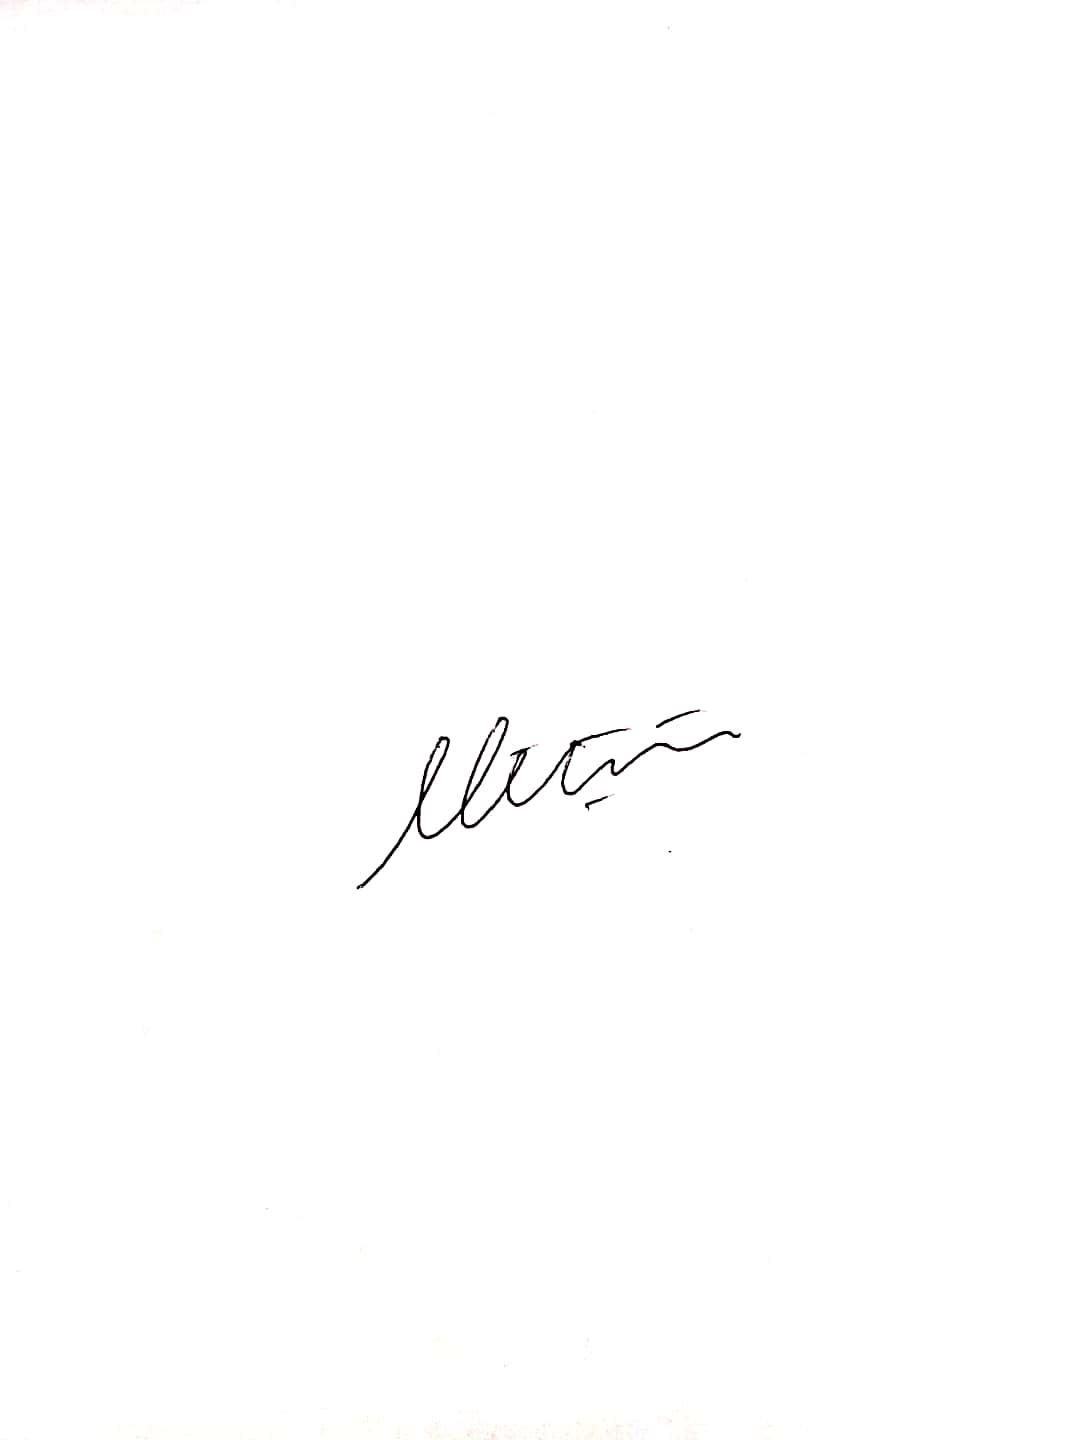
\includegraphics[height=2cm]{signature}\\
\fromsig{Kathryn Huff\\Assistant Professor\\Nuclear, Plasma, \& Radiological 
Eng.\\University of Illinois\\kdhuff@illinois.edu}
}

%----------------------------------------------------------------------------------------

\end{letter}

\end{document}


